\newpage
\chapter{Automation and Scripting}
Often a user will have set up a simulation structure to represent a real world device but will then ask the question: What happens to my solar cell efficiency as I change the mobility of the active layer? Or what happens to the wavelength of my laser output as I change the thickness of the Quantum Well. To answer these type of questions one must change one or more material parameters over a range of values and then examine the simulation results.  Clearly this could be done by hand but there are better ways to automate this process.

There are three main ways to automate OghamNano simulations:
\begin{enumerate}
  \item The first method is using the parameter scan window, this is described below in section \ref{sec:scanwindow}.  The parameter scan window allows a user to vary a parameter (or multiple paramters) in steps using the graphical user interface. No knowledge of coding is required for this approach.  The parameter scan window is useful if one wants to quickly examine how a parameter influences the results and the scenario you are examining is not very complex. The scan window fits most users's needs most of the time.
  \item For more fine grained control over how the parameters are varied the next method is to use Python scripting, this is described in section \ref{sec:pythonscripts}.  Python scripting allws the user ultimate flexibility in adjusting all simulation parameters and running simulations, Python is widely available which makes this approach very attractive. 
  \item The third way is through MATLAB scripting, this is described in section \ref{sec:matlabscripts}. The advantage of MATLAB scripting is that lots of people can code in MATLAB so makes automating OghmaNano very accessable. The downside of using MATLAB is that it is quite expensive and not all people have access to it. An alternative to MATLAB would be Octave however at the time of writing it does not have a json reader/writer.
\end{enumerate}

Or option 4: All the above methods rely on the same principles: The OghmaNano simulation save file is systematic edited and the back end of the software $oghma\_core.exe$ run on the sim.oghma file to generate new results. Key to understanding how scripting works is to realize that the sim.oghma is simply a zip file (See \ref{sec:fileformat}) with a json file (sim.json) inside it, and if one can edit the json file (using any language you want ActionScript, C, C++, C\#, Cold Fusion, Java, Lisp, Perl, Objective-C, OCAML, PHP, Python, Ruby etc... ) the you can automate OghmaNano.
\vfill

\pagebreak
\section{The parameter scan window}
\label{sec:scanwindow}
Related YouTube videos:
\begin{figure}[H]
\begin{tabular}{ c l }

\includegraphics[width=0.05\textwidth]{./images/youtube.png}
&
\href{https://www.youtube.com/watch?v=cpkPht-CKeE}{Using the parameter scan tool in OghmaNano}
\end{tabular}
\end{figure}

\vspace{0pt}
\noindent
\begin{minipage}{0.5\textwidth}
The most straight forward way to systematically vary a simulation parameter is to use the scan window. In this example we are going to systematic change the mobility of the active layer of a PM6:Y6 solar cell, you can find this example in the example simulations under \emph{Scripting and fitting/Scan demo (PMY:Y6 OPV)}. Once you have located this simulation and opened it, you then need to bring up the parameter scan window, this can be done by clicking on the \emph{Parameter scan} icon in the Automation ribbon (see Figure \ref{fig:parameter_scan_icon}).  Then make a new scan by clicking on the \emph{new scan} button (1) (In the example simulation this has already been done for you). Open the new scan by double clicking on the icon representing the scan (2), see figure \ref{fig:newscan}. This will bring up the scan window, see figure \ref{fig:newscanline}.
\end{minipage}% Don't leave empty lines and empty chars between minipages
\hspace{4pt}
\begin{minipage}[]{0.5\linewidth}
\centering
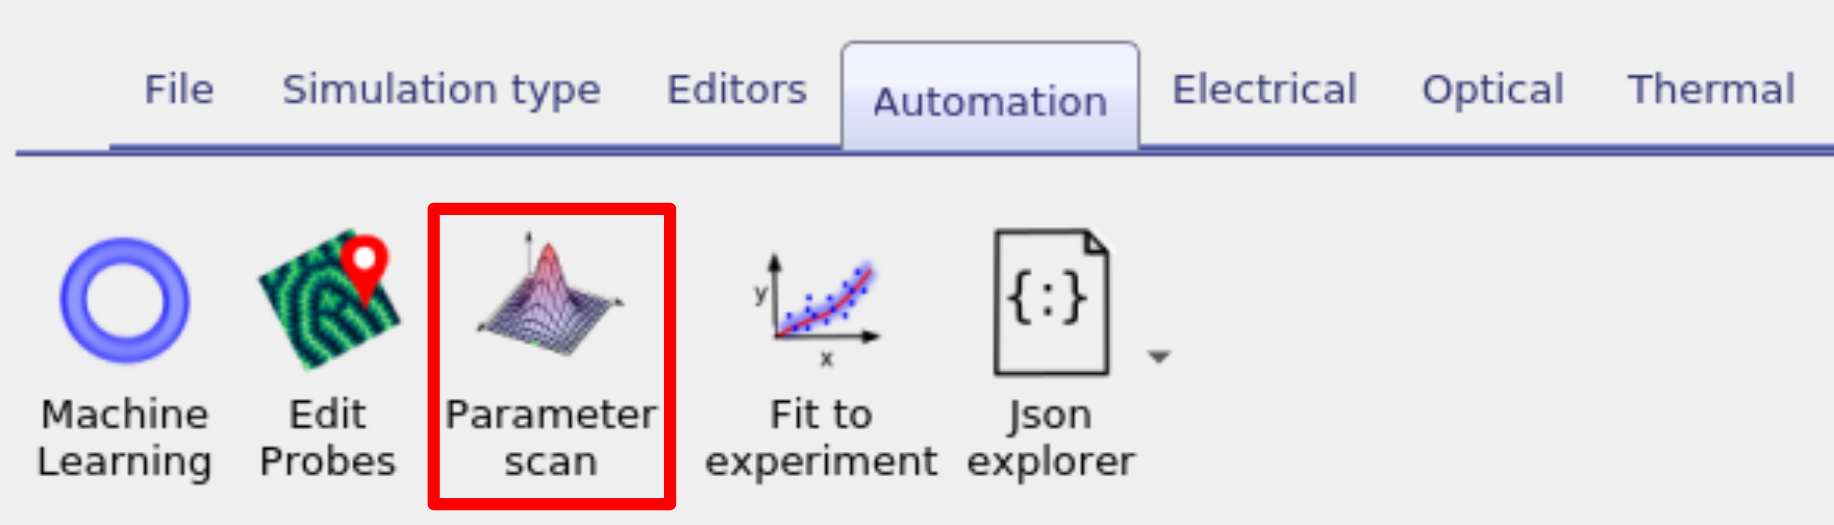
\includegraphics[width=\textwidth]{./images/param_scan.png}
\captionof{figure}{Step 1: Select the Parameter scan tool, to bring up the parameter scan window.}
\label{fig:parameter_scan_icon}

\centering
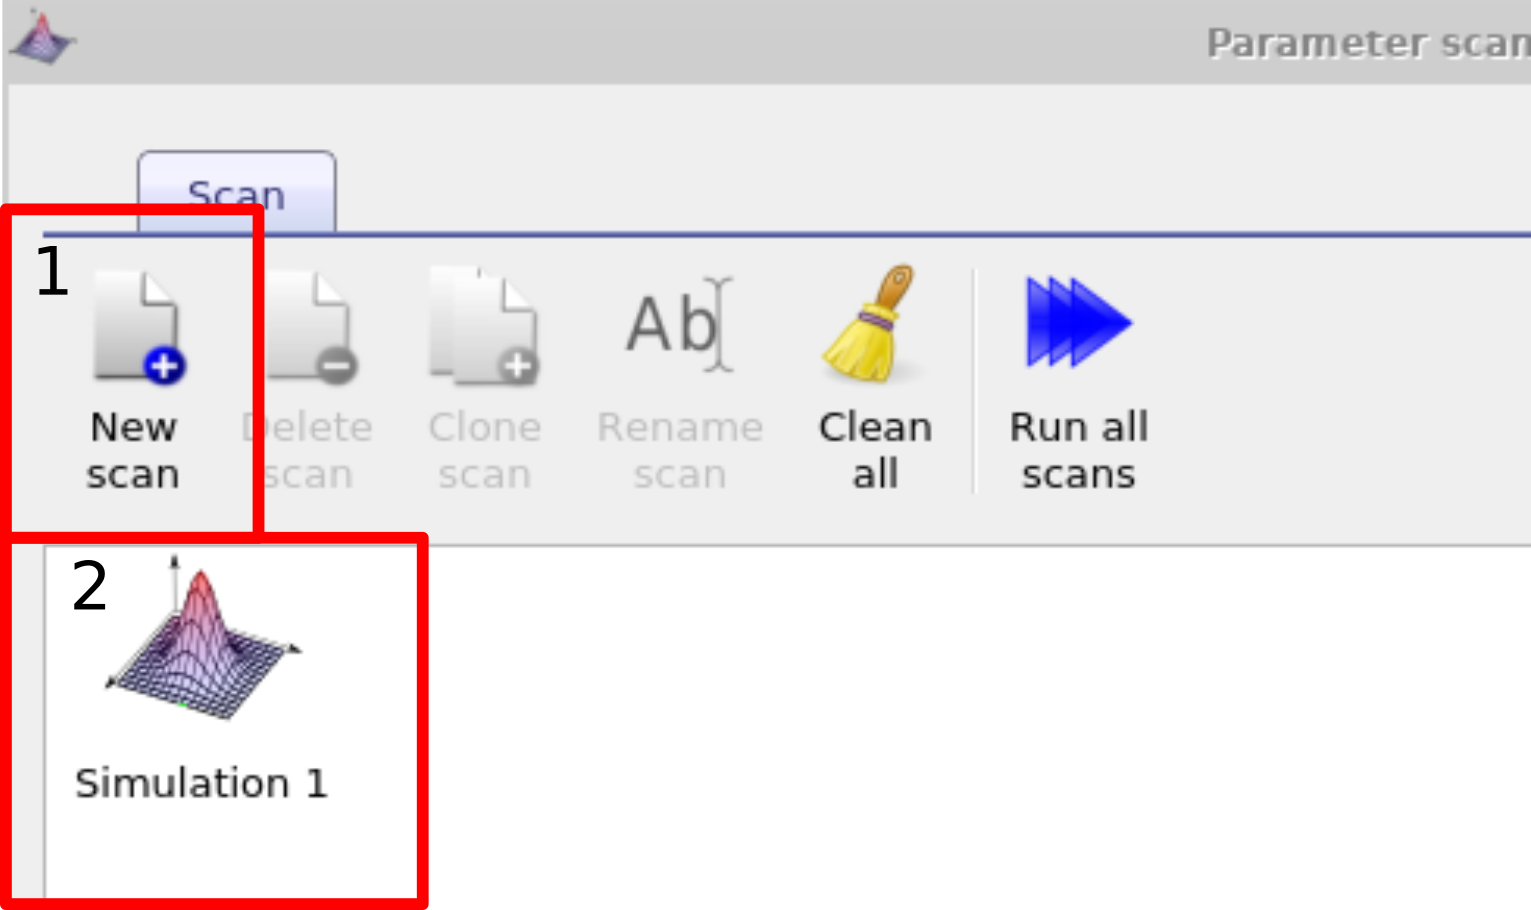
\includegraphics[width=\textwidth]{./images/param_scan_new.png}
\captionof{figure}{Step 2: Make a new parameter scan, then double click on it to open it.}
\label{fig:newscan}

\end{minipage}

\subsection{Changing one material parameter}
Once the \emph{scan window} has opened, make a new scan line by clicking on the the plus icon (1) in figure \ref{fig:newscanline}, then select this line so that it is highlighted (2), then click on the three dots (3) to select which parameter you want to scan. Again if you are using the example simulation this will already have been done for you.

\begin{figure}[H]
\centering
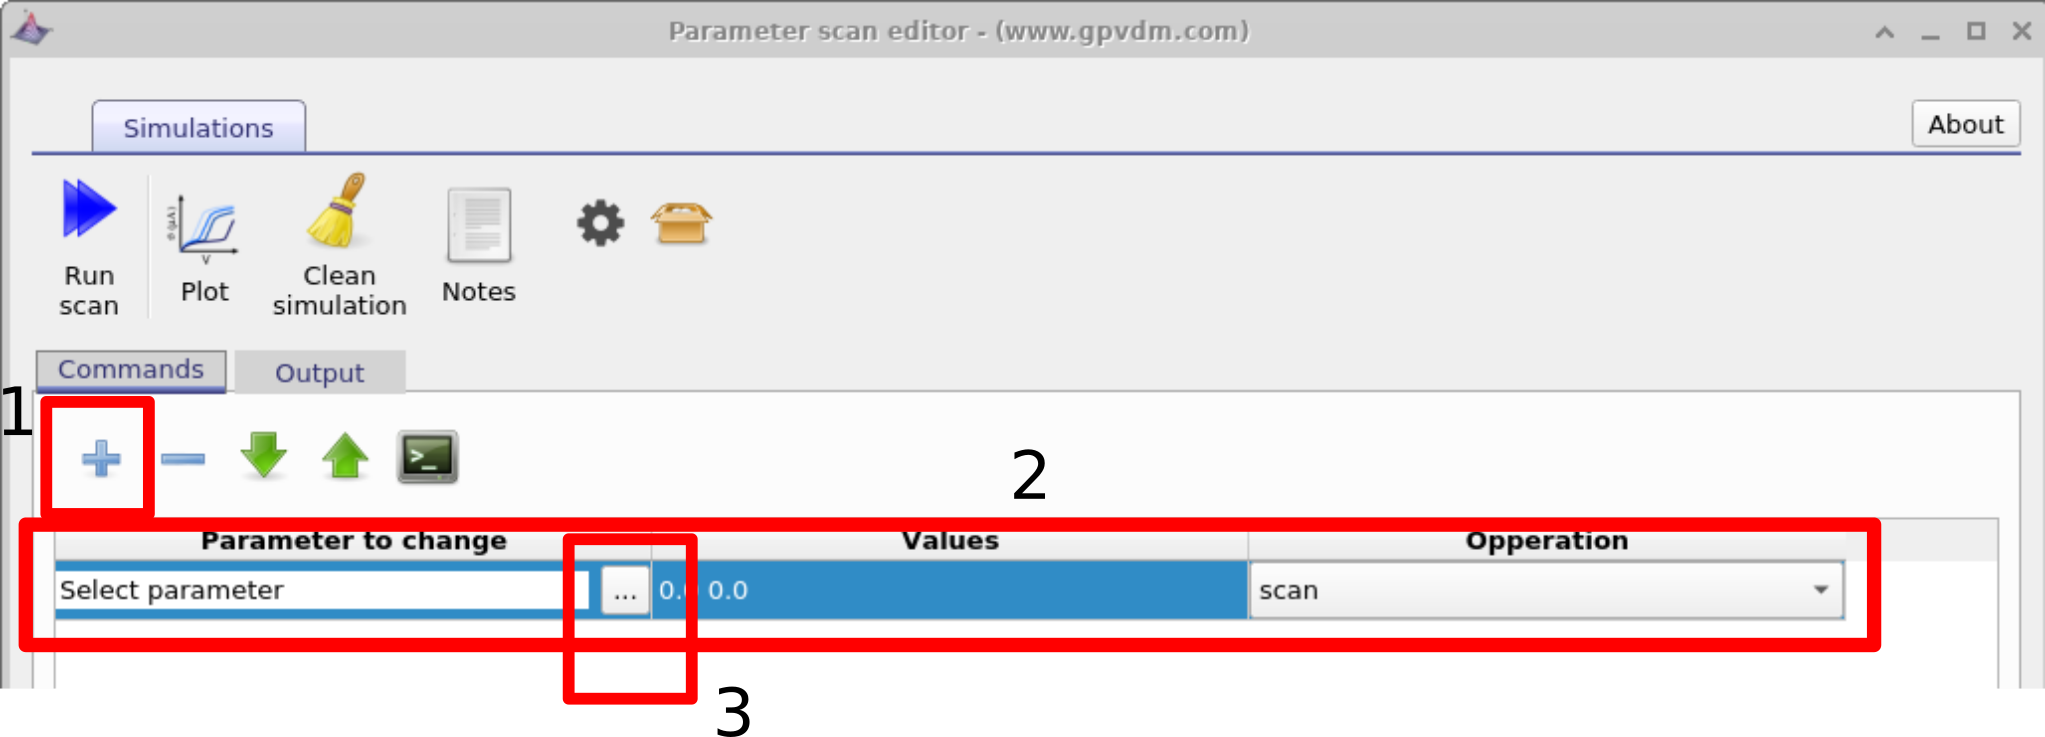
\includegraphics[width=\textwidth]{./images/param_scan_new_line.png}
\caption{Step 3: Add a 'scan line' to the scan.}
\label{fig:newscanline}
\end{figure}
\pagebreak
\noindent
\begin{minipage}{0.5\textwidth}

In this example we will be selecting the electron mobility of a PM6:Y6 solar cell. Do this by navigating to epitaxy$\rightarrow$ PM6:Y6$\rightarrow$ Drift diffusion$\rightarrow$ Electron mobility y. Highlight the parameter and then click OK. This should then appear in the scan line. The meaning of \emph{epitaxy$\rightarrow$ PM6:Y6$\rightarrow$ Drift diffusion$\rightarrow$Electron mobility y} will now be explained below:

\begin{itemize}
  \item epitaxy: All parameters in the .oghma file are exposed via the parameter selection window see \ref{fig:scanselect}. This file is a tree structure, see \ref{sec:fileformat}. The device structure is defined under the heading epitaxy.
  \item PM6:Y6: Under epitaxy each layer of the device is given by its name. The active layer in this device is called PM6:Y6, if your active layer was called Perovskite or P3HT:PCBM you would have selected this instead.
  \item Drift diffusion: All electrical parameters are stored under the sub heading \emph{drift diffusion}.
\end{itemize}

\end{minipage}% Don't leave empty lines and empty chars between minipages
\hspace{4pt}
\begin{minipage}[]{0.5\linewidth}
\centering
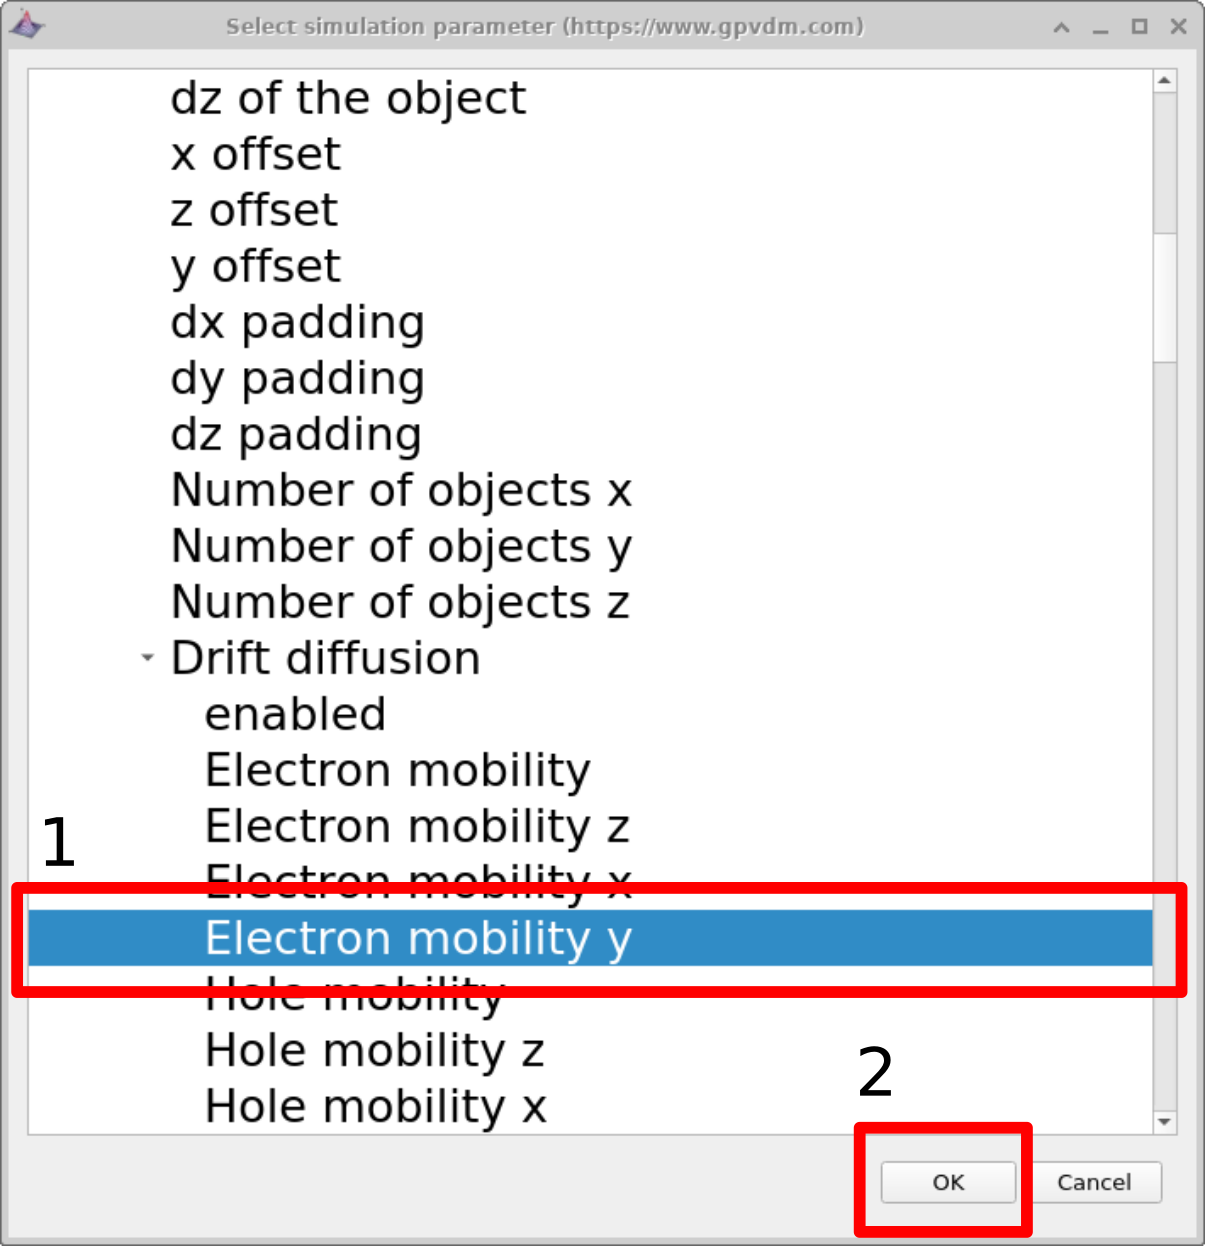
\includegraphics[width=\textwidth]{./images/param_scan_select.png}
\captionof{figure}{Step 5: Select the parameter you want to scan in the parameter selection window, in this case we are selecting epitaxy$\rightarrow$ PM6:Y6$\rightarrow$ Drift diffusion$\rightarrow$ Electron mobility y.}
\label{fig:scanselect}

\end{minipage}

\begin{itemize}

  \item Electron mobility y: One can define asymmetric mobilities in the z,x and y direction - this is useful for OFET simulations.  However by default the model assumes a symmetric mobility which is the same in all directions. This value is defined by \emph{Electron mobility y}. 
\end{itemize}

Next enter the values of mobility which you want to scan over in this case we will be entering \emph{1e-5 1-6 1e-7 1e-8 1e-9} (see figure \ref{fig:runscan} 1) then click \emph{run scan} (see figure \ref{fig:runscan} 2). OghmaNano will run one simulation on each core of your computer until all the simulations are finished.

\begin{figure}[H]
\centering
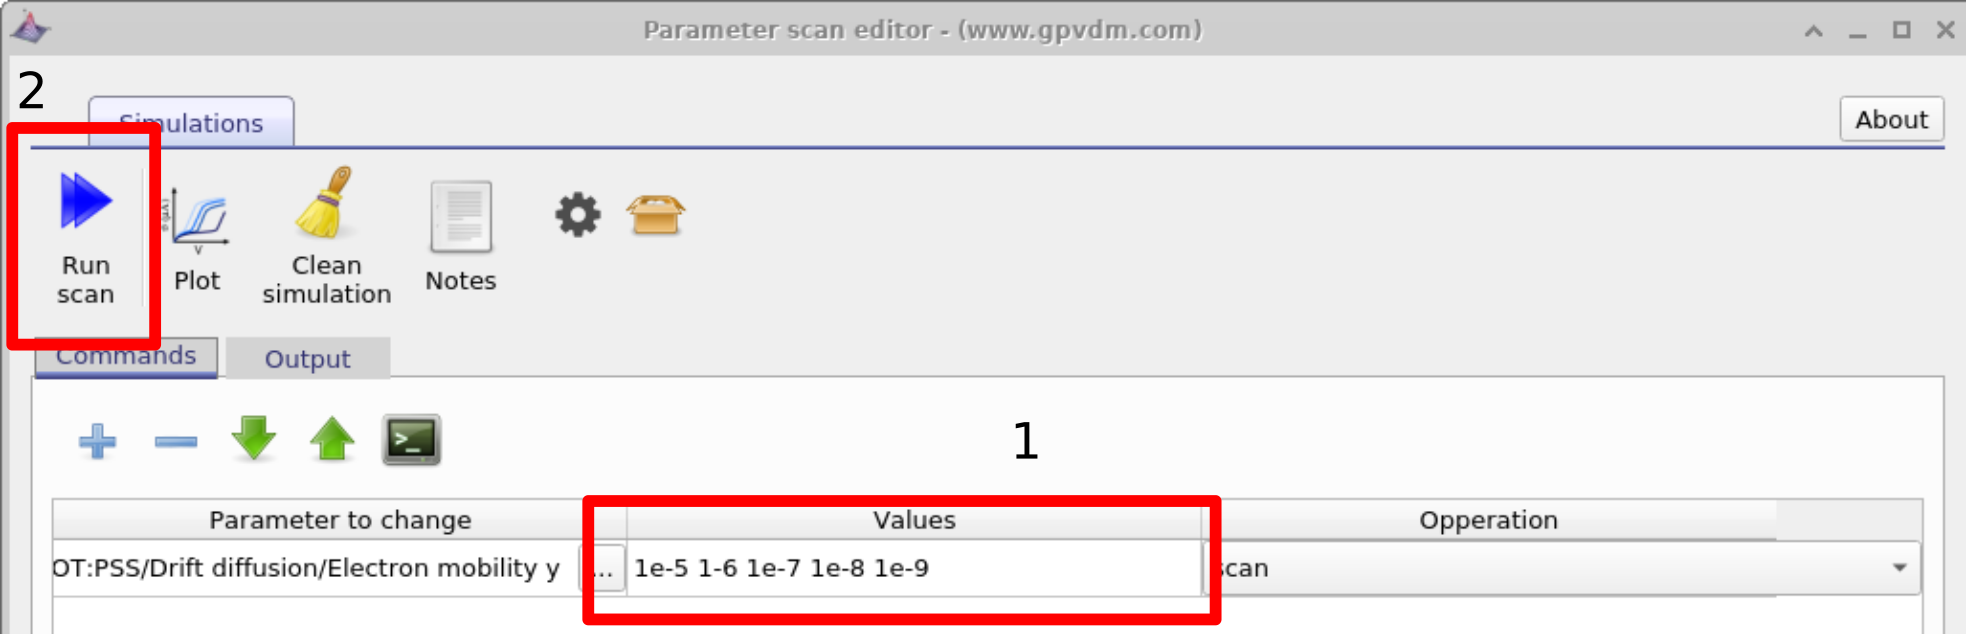
\includegraphics[width=0.8\textwidth]{./images/param_scan_inputvalues.png}
\caption{Step 6: Enter the input values of mobility (or other values) you want to scan over (1). Then run the simulations.}
\label{fig:runscan}
\end{figure}

To view the simulation results click on the \emph{output} tab this will bring up the simulation outputs, see figure \ref{fig:scanoutput}. You can see that a directory has been created for each variable that we scanned over so \emph{1e-5, 1e-6, 1e-7, 1e-8 and 1e-9}.  If you look inside each directory it will be an exact copy of the base simulation directory.  If you double click on the files with multi-colored JV curves, see the red box in figure \ref{fig:scanoutput}. OghmaNano will automaticity plot all the curves from each simulation in one graph, see figure \ref{fig:scanjv}.

\begin{figure}[H]
\centering
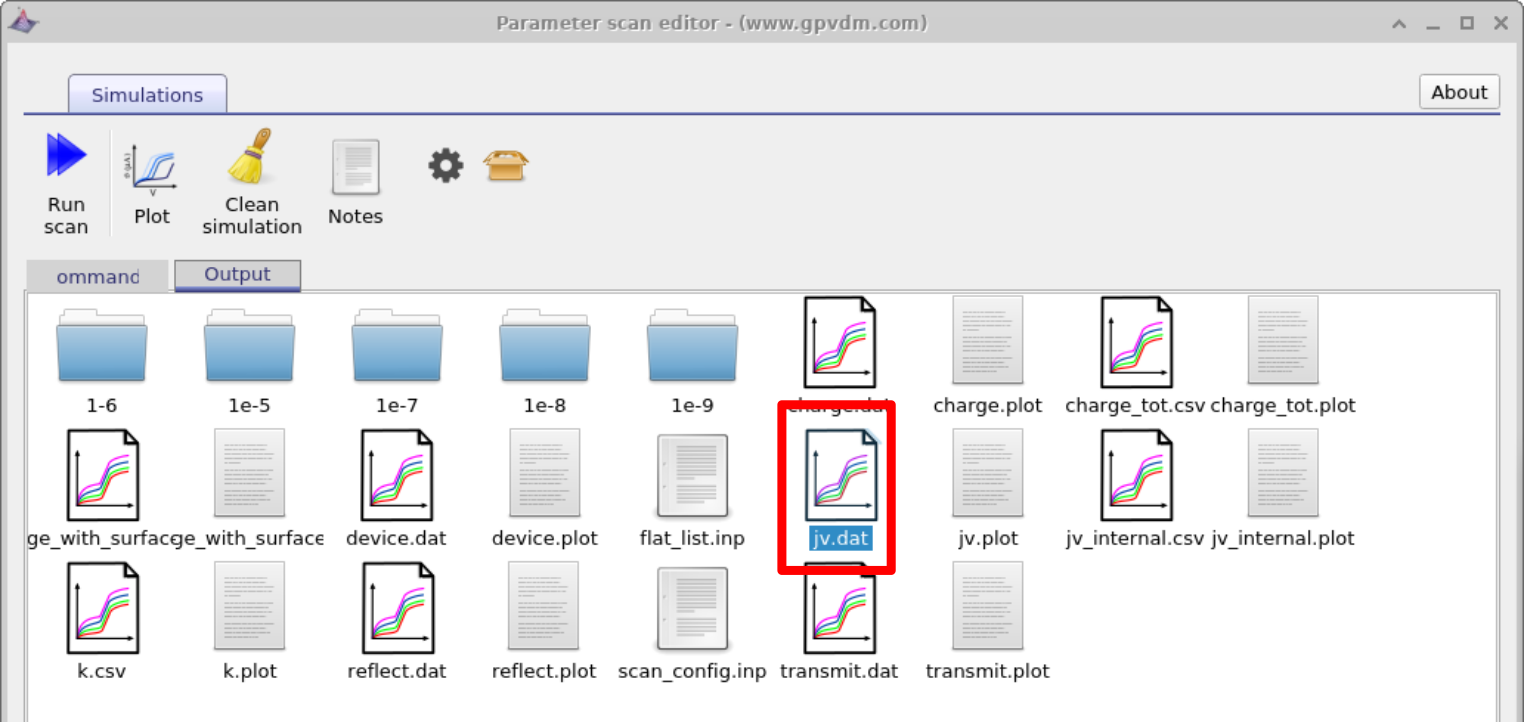
\includegraphics[width=\textwidth]{./images/param_scan_output.png}
\caption{Step 7: The output tab showing the five simulation directories and the multicolored plot files.}
\label{fig:scanoutput}
\end{figure}

\begin{figure}[H]
\centering
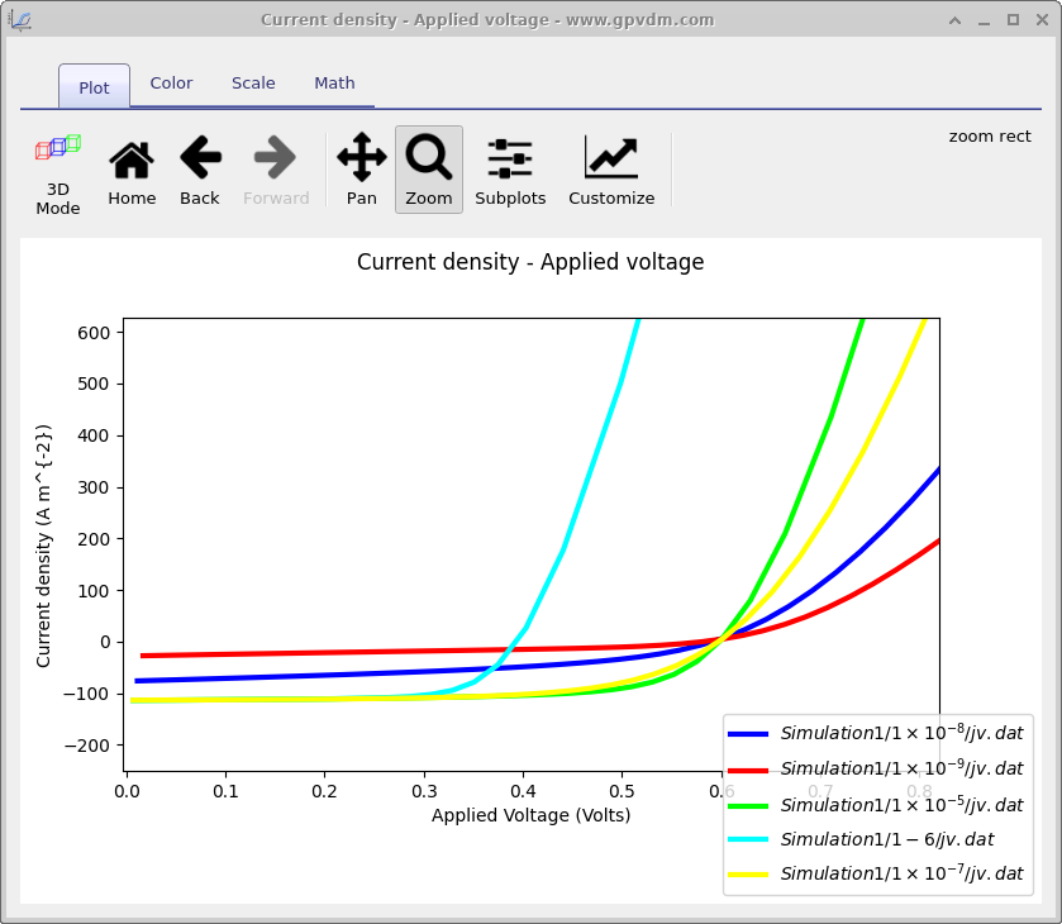
\includegraphics[width=0.5\textwidth]{./images/param_scan_jv.png}
\caption{Step 8: The result of the mobility scan.}
\label{fig:scanjv}
\end{figure}

\subsection{Duplicating parameters - changing the thickness of the active layer}

Very often one wants to change a parameter, then set another parameter equal to the parameter which was changed. An example of this is one may want to change electron and hole mobilities together when simulating a device with symmetric mobilities. This can be done using the duplicate function of the scan window as seen in figure \ref{fig:scanduplicate}.  In this example we tackle a slightly more tricky problem than changing mobilities together we are going to change the physical width of the active layer and at the same time adjust the electrical mesh to make it match.  As discussed in section \ref{ref:mesh} the width of the active layer must always match the width of the electrical mesh.  When you change the layer width by hand in the layer editor OghmaNano updates the width of the electrical mesh for you. But when scripting the model it won't do this update for you.  Therefore in the example below we are going to set the width of the active layer by scanning over:

epitaxy$\rightarrow$PM6:Y6$\rightarrow$dy of the object
\\
\\
Then we are going to add another line under and under parameter to scan select
\\
\\
mesh$\rightarrow$mesh\_y$\rightarrow$segment0$\rightarrow$len
\\
\\
and set it to
\\
\\
epitaxy$\rightarrow$PM6:Y6$\rightarrow$dy of the object
\\
\\
under the operation dropdown box. You will see the word duplicate appear under values.
\\
\\
If you now run the simulation "epitaxy$\rightarrow$PM6:Y6$\rightarrow$dy of the object" will be changed and "mesh$\rightarrow$mesh\_y$\rightarrow$segment0$\rightarrow$len" will follow it.


\begin{figure}[H]
\centering
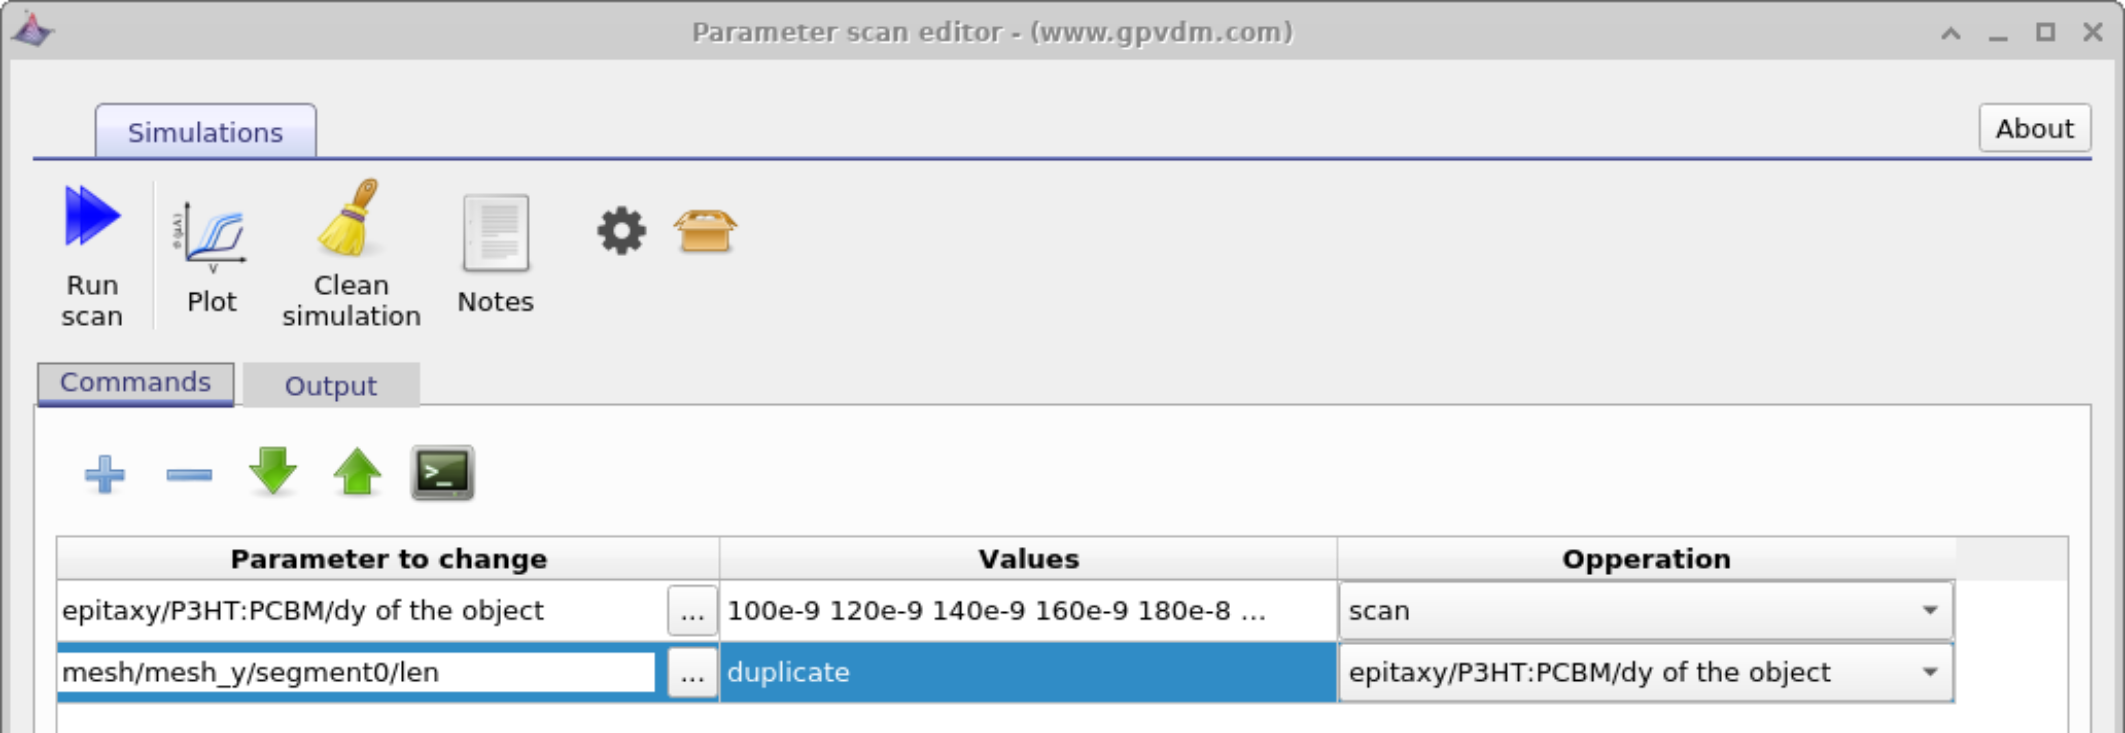
\includegraphics[width=0.7\textwidth]{./images/param_scan_duplicate.png}
\caption{Duplicating material paramters.}
\label{fig:scanduplicate}
\end{figure}

\subsubsection{Side note: Device with multiple active layers}
The sum of the active layer thickness (as defined in the layer editor) MUST equal the electrical mesh thickness (more about the mesh in section \ref{ref:mesh}).  If for example one had three active layers TiO2 (100 nm)/Perovskite (200 nm)/Spiro (100 nm) with a total width of 400 nm.
The total mesh length must be 400 nm as well.  Therefore were one want to change the thickness of the perovskite layer as in \ref{fig:scanduplicate} one would have to break the electrical mesh up into three sections and make sure you were updating the mesh segment referring to the perovskite layer alone.

\subsection{Setting constants}
Often when running a parameter scan one wants to set a constant value, this can be done using the "constant" option in the Operations dropdown menu. See figure \ref{fig:scanconst}

\begin{figure}[H]
\centering
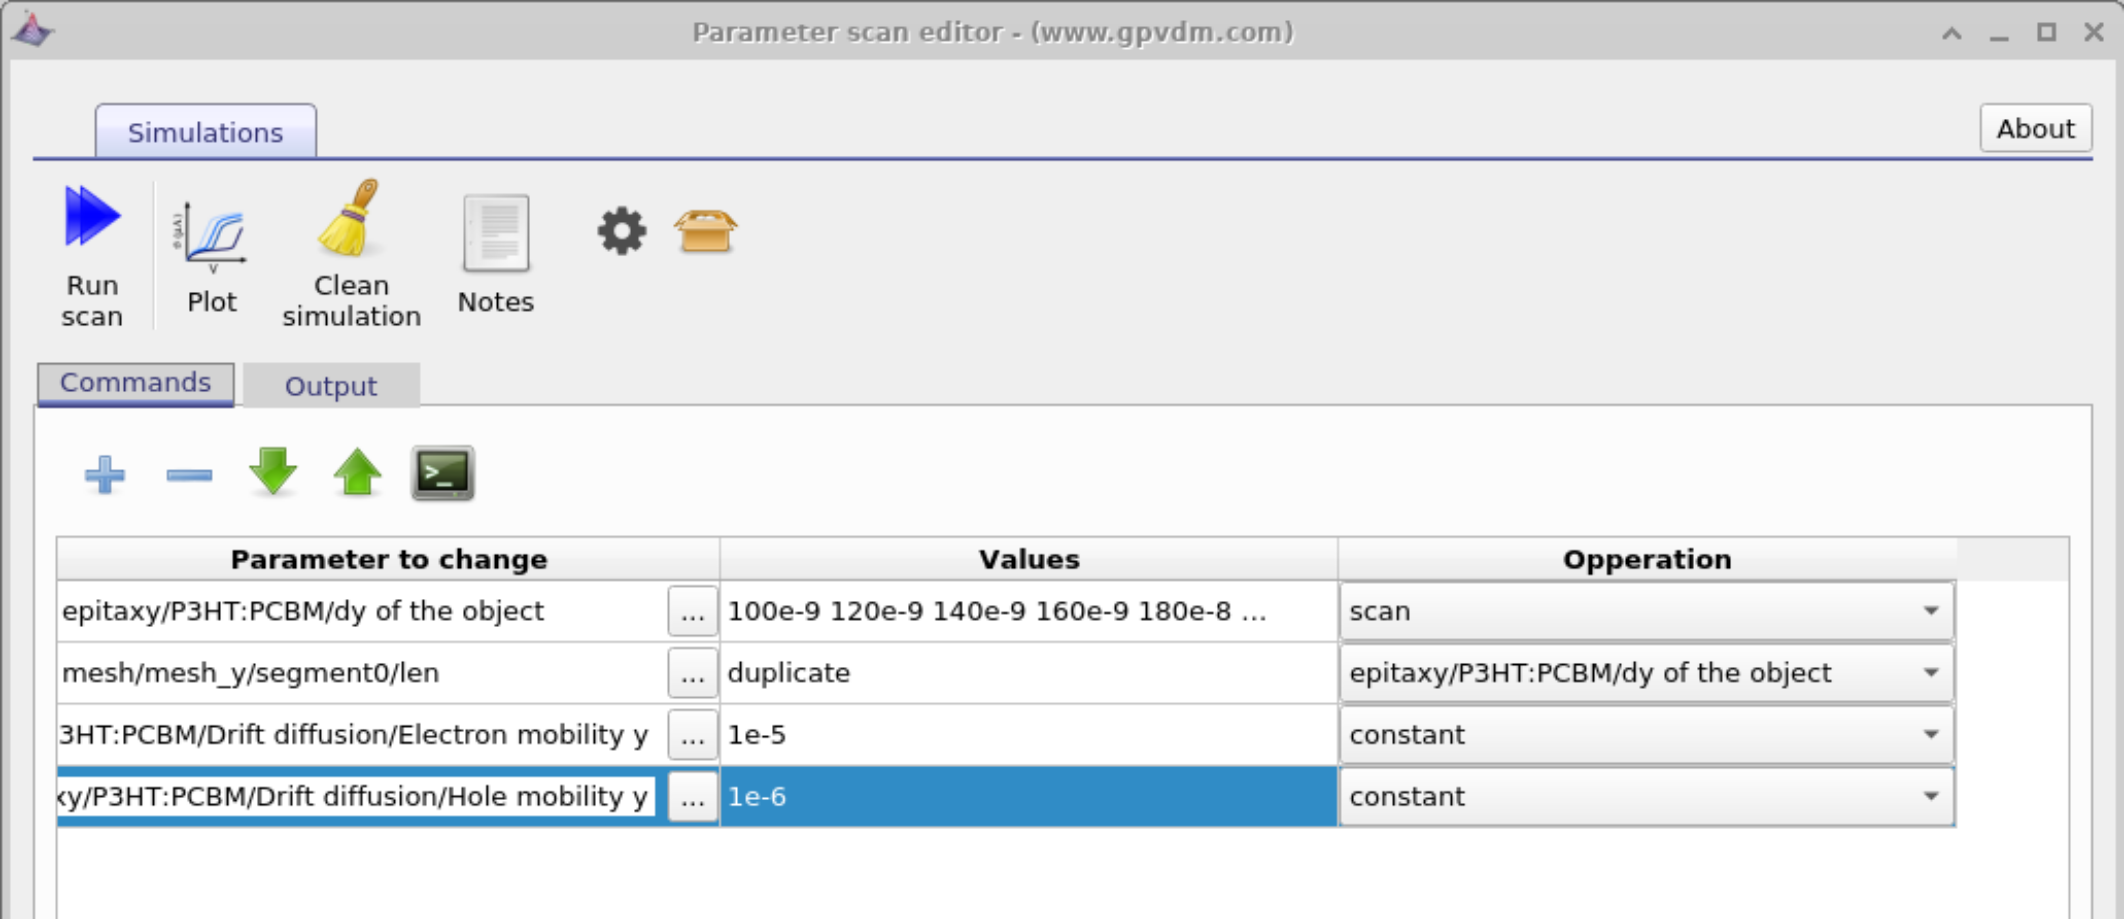
\includegraphics[width=0.5\textwidth]{./images/param_scan_const.png}
\caption{The result of the mobility scan.}
\label{fig:scanconst}
\end{figure}

\subsection{The equivalent of loops}
Often when scanning over a parameter range one may want to simulate so many parameters that it is not practical to type them in.  In this case OghmaNano has the equivalent of a loop. So for example if one wanted to change a value from 100 to 400 in steps of 1, one could type

\begin{listing}[H]
\begin{minted}[frame=single,
               framesep=3mm,
               linenos=false,
               xleftmargin=21pt,
               tabsize=4]{matlab}

[100 400 1]

\end{minted}
\caption{The equivalent of loops in OghmaNano, this is often quicker than typing parameters in by hand.} 
\label{json-example}
\end{listing}

\subsection{Limitations of the scan window}
Although the scan window is convenient in that it provides a quick way to scan simulation parameters, it is by nature rather limited in terms of flexibility. If you want to do complex scans were multiple parameters are changed or to programmatically collect data from each simulation then you can use the \index{python} or matlab interfaces to OghmaNano.  These are described in the latter sections.
\vfill

\pagebreak
\section{Multiparameter device optimizer}
\label{sec:device_optimizer}
Related YouTube videos:

\begin{figure}[H]
\begin{tabular}{ c l }

\includegraphics[width=0.05\textwidth]{./images/youtube.png}
&
\href{https://www.youtube.com/watch?v=L5o0ogp67vE}{Optimizing the layer structure of a Perovskite solar cell}
\end{tabular}
\end{figure}

\begin{figure}[H]
\begin{tabular}{ c l }


\includegraphics[width=0.05\textwidth]{./images/youtube.png}

&
\href{https://www.youtube.com/watch?v=sBhCg9lWjZ8 }{Optimizing an OPV device for maximum photon harvesting.}

\end{tabular}
\end{figure}

\begin{figure}[H]
\begin{tabular}{ c l }


\includegraphics[width=0.05\textwidth]{./images/youtube.png}

&
\href{https://www.youtube.com/watch?v=60RVozhJqFY  }{Searching for the optimum layer structure in an organic solar cell.}

\end{tabular}
\end{figure}

Very often when optimizing a device an engineer or scientists will be want to know what the optimum structure of a device is. For example a perovskite solar cell is made up of multiple layers, but what is the optimum thickness of each layer? If the perovskite layer is made really thick then lots of light will be absorbed but the down side of this is that it will take longer for charge carriers to escape the device so recombination will be high.  Conversely if the layer is made really thin very few carriers will have a chance to recombine as they will not spend long in the device but the downside is that not many photons will be absorbed in the first place as the layer is thin.  If one then also considers that light will reflect multiple times of interfaces in the device setting up standing wave pattens, this will further complicate the optimization problem as one will need to optimize not only the thickness of the perovskite layer but also the thicknesses of all other layers at the same time. To solve this multi-parameter optimization problem one can use the \emph{Fast optimizer} within the scan window.

\subsection{Using the multi parameter optimizer}
In the new simulation window under the sub-topic \emph{Scripting and fitting} there are several examples of multi-parameter optimizers:

\begin{itemize}
  \item Electrical layer optimizer: This will vary the layer thickness of two active layers of an organic solar cell simulation and plot the PEC/FF/Voc as a function of these layer thicknesses.
  \item Optical layer optimizer (perovskite): This will vary the thickness of two layers in a perovskite solar cell and plot the current generated by each layer within the device.
  \item Optical layer optimizer (OPV): This will vary the thickness of two layers in a perovskite solar cell and plot the current generated by each layer within the device.
\end{itemize}

In this text we will be using the \emph{Optical layer optimizer (perovskite)}, if you open this simulation and navigate to the scan window, you will see a scan already set up called \emph{optimizer}. If you open it you will get a window shown in figure \ref{fig:device_optimizer}. This scan window looks just like the scan windows described in the previous section, however the key difference is that the \emph{Fast optimizer} button is depressed. When this button is depressed scan results are not written to disk, instead the key simulation parameters are tabulated and saved to disk at the end of the simulation.  Notice that in this example we are varying the thickness (dy) of the Perovskite layer between 300nm and 500 nm in steps of 10 nm and the thickness (dy) TiO2 layer from 100 nm to 300 nm also in steps of 10 nm. Try running the simulation, the using windows explorer navigate to your simulation directory, then open the folder called \emph{optimize} and in there you will find a \emph{csv} file called \emph{optimizer\_output.csv}. If you open this with Excel or LibreOffice, it will look like figure \ref{fig:device_optimizer_output}.

\begin{figure}
\centering
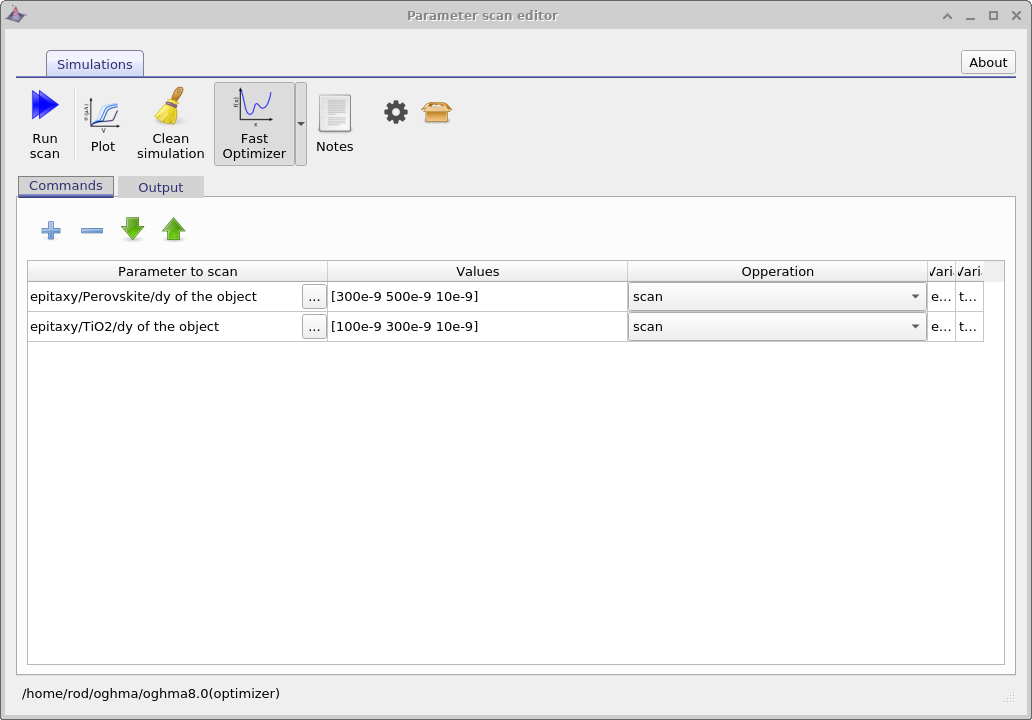
\includegraphics[width=0.6\linewidth,height=0.5\linewidth]{./images/scan_optimizer.png}
\caption{The scan window with the optimizer button depressed ready to run a device layer optimization.}
\label{fig:device_optimizer}
\end{figure}

If you examine figure \ref{fig:device_optimizer_output} carefully you can see the first two columns are labelled epitaxy.layer2.dy and epitaxy.layer1.dy . These are the layer thicknesses we decided to change in the scan window.  For every subsequent layer in the device there are two columns, labelled layerX/light\_frac\_photon\_generation and layerX/J. These refer to the fraction of the light absorbed with in the layer and the maximum current this layer would produce if all the light absorbed within the layer were turned into current. Clearly if light is absorbed within the active layer it has a good chance of being turned into current, however if light is absorbed within the back metallic contact  then there is little chance of that light being turned into electrical current. If you use the sorting tools included within Excel/LibreOffice you can figure out which device structures produce the most current.

\begin{figure}
\centering
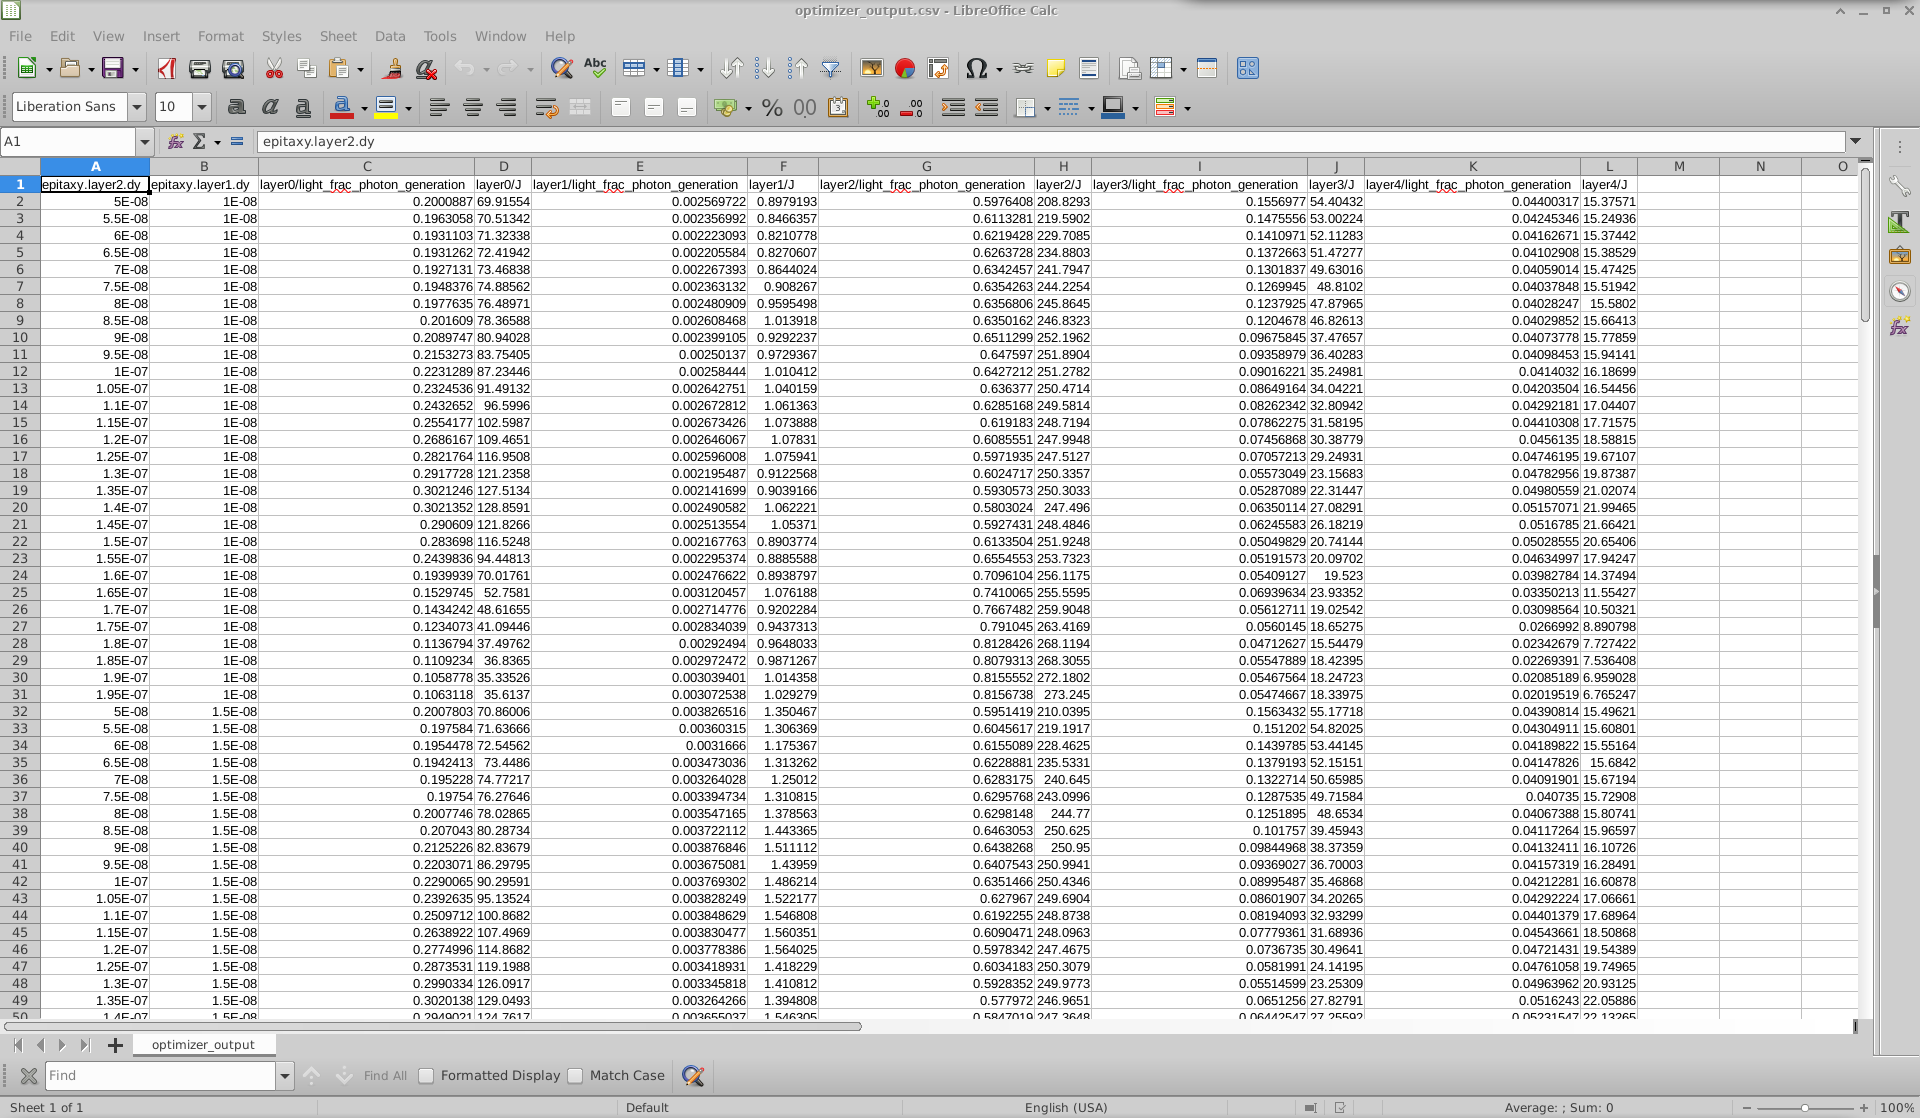
\includegraphics[width=\linewidth]{./images/scan_optimizer_output.png}
\caption{The file your simulation directory/optimizer/optimizer\_output.csv} opened in LibreOffice (You can use Excel).
\label{fig:device_optimizer_output}
\end{figure}
\vfill

\pagebreak
\section{Python/MATLAB scripting of OghmaNano}
Scripting offers a more powerful way to interact with gvpdm. Rather than using the graphical user interface, you can use your favourite programming language to interact with OghmaNano.  This gives you the option to drive simulations in a far more powerful way than can be done using the graphical interface alone.  Below I give examples of using MATLAB and python to drive OghmaNano, but you can use any language you want which has a json reader/writer.  Pearl and Java are two languages which spring to mind.

Before you begin scripting OghmaNano you need to tell windows where OghmaNano is installed, the default OghmaNano will be installed to C:\textbackslash Program files x86 \textbackslash OghmaNano, in there you will see in this directory there are two windows executables, one called \emph{oghma.exe}, this is the graphical user interface, and a second .exe, called \emph{oghma\_core.exe}.  You can run \emph{oghma\_core.exe} from the command line without \emph{oghma.exe}. You simply need to navigate to a directory containing a \emph{sim.oghma} folder and call \emph{oghma\_core.exe}, this can be done from the windows command line, matlab, python or any other scripting language.
However, before you can do this on windows, you need to add C:\textbackslash Program files x86 \textbackslash OghmaNano to your windows path so that windows knows where OghmaNano is installed.  An example of how to do this on a modern version of windows is given in the link
\url{https://docs.microsoft.com/en-us/previous-versions/office/developer/sharepoint-2010/ee537574(v=office.14)}

Every new version of windows seems to move the configuration options around, so you may have to find instructions for your version of windows.

\subsection{Python scripting}
\label{sec:pythonscripts}
Related YouTube videos:
\begin{figure}[H]
\begin{tabular}{ c l }


\includegraphics[width=0.05\textwidth]{./images/youtube.png}

&
\href{https://www.youtube.com/watch?v=vyeAzxBZjMg}{Python scripting perovskite solar cell simulation}

\end{tabular}
\end{figure}

There are two ways to interact with \fileext files via python, using native python commands or by using the \simname class structures, examples of both are given below.


\subsubsection{The native python way}
As described in section \ref{sec:fileformat}, \fileext files are simply json files zipped up in an archive. If you extract the sim.json file form the sim\fileext file you can use Python's json reading/writing code to edit the .json config file directly, this is a quick and dirty approach which will work. You can then use the $os.system$ call to run oghma\_core to execute \simname.

For example were one to want to change the mobility of the 1st device layer to 1.0 and then run a simulation you would use the code listed in listing \ref{python-example}.

\begin{listing}
\begin{minted}[frame=single,framesep=3mm,linenos=false,xleftmargin=21pt,tabsize=4]{python}

	import json
	import os
	import sys

	f=open('sim.json')		#open the sim.json file
	lines=f.readlines()
	f.close()
	lines="".join(lines)	#convert the text to a python json object
	data = json.loads(lines)

	#Edit a value (use firefox as a json viewer
	# to help you figure out which value to edit)
	# this time we are editing the mobility of layer 1
	data['epitaxy']['layer1']['shape_dos']['mue_y']=1.0


	#convert the json object back to a string
	jstr = json.dumps(data, sort_keys=False, indent='\t')

	#write it back to disk
	f=open('sim.json',"w")
	f.write(jstr)
	f.close()

	#run the simulation using oghma_core
	os.system("oghma_core.exe")
\end{minted}
\caption{Manipulating a sim.json file with python and running a \simname simulation.} 
\label{python-example}
\end{listing}

If the simulation in sim.json is setup to run a JV curve, then a file called sim\_data.dat will be written to the simulation directory containing paramters such as PCE, fill factor, $J_{sc}$ and $V_{oc}$.  This again is a raw json file, to read this file in using python and write out the value of $V_oc$ to a second file use the code given in listing \ref{python-example2}.

\begin{listing}
\begin{minted}[frame=single,framesep=3mm,linenos=false,xleftmargin=21pt,tabsize=4]{python}
f=open('sim_info.dat')
lines=f.readlines()
f.close()
lines="".join(lines)
data = json.loads(lines)

f=open('out.dat',"a")
f.write(str(data["Voc"])+"\n");
f.close()

\end{minted}
\caption{Reading in a sim\_data.dat file using Python's native json reader.} 
\label{python-example2}
\end{listing}



\subsubsection{Using \simname's built in classes for reading and writing json}
\simname has a set of classes that can read in \simname files and write them to disk. The difference between using python's native commands and the gpvmd classes is that, \simname will convert the json save files to a hierarchical tree of python classes rather than leaving them as raw json. So for example using Python's native json interpreters one would write:

 
\begin{listing}
\begin{minted}[frame=single,framesep=3mm,linenos=false,xleftmargin=21pt,tabsize=4]{python}
	data['epitaxy']['layer1']['shape_dos']['mue_y']=1.0
\end{minted}
\caption{Reading in a sim\_data.dat file using Python's native json reader.} 
\label{python-example3}
\end{listing}

but using the \simname interpreter one would write

\begin{listing}
\begin{minted}[frame=single,framesep=3mm,linenos=false,xleftmargin=21pt,tabsize=4]{python}
	data.epitaxy.layer[1].shape_dos.mue_y=1.0
\end{minted}
\caption{Reading in a sim\_data.dat file using Python's native json reader.} 
\label{python-example4}
\end{listing}

The \simname class tree also has embedded functions for searching for objects and alike some of which are described below in listing \ref{python-example5}.

\begin{listing}
\begin{minted}[frame=single,framesep=3mm,linenos=false,xleftmargin=21pt,tabsize=4]{python}
#!/usr/bin/env python3
import json
import os
import sys

sys.path.append('c:\Program files x86\\simname\modules')
from json_root import json_root

data=json_root()
data.load("sim.json")
data.epitaxy.layer[1].shape_dos.mue_y=1.0
data.save()

os.system("coreexename.exe")

\end{minted}
\caption{Editing sim.json files using \simname's built in classes.} 
\label{python-example5}
\end{listing}

\subsubsection{Running \simname across multiple cores}
The scan window by default uses \simname's built in job scheduler so that if you want to scan across 10 parameters and have a CPU with multiple cores, the jobs will be spread across all cores.  This increases the overall speed of the simulations. You can access this API using the \simname\_api class, an example of how to do this is given in listing \ref{python-example6}.

\begin{listing}
\begin{minted}[frame=single,framesep=3mm,linenos=false,xleftmargin=4pt,tabsize=4]{python}
#!/usr/bin/env python3
import os
import sys
sys.path.append('c:\Program files x86\ \simname \ modules')

from model_api import model_api

#initialize the API
api=model_api(verbose=False)

#Use the name of the current script to determine the directory name to make
script_name=os.path.basename(__file__).split(".")[0]

#define the name of the simulation dir
scan_dir=os.path.join(os.getcwd(),script_name)

#make the simulation dir
api.mkdir(scan_dir)					#make a new scandir

#tell the API where we are going to run the simulation
api.server.server_base_init(scan_dir)

#Loop over electron and hole mobilities.
for mue in [ 1e-5, 1e-6, 1e-7, 1e-8]:
	for muh in [ 1e-5, 1e-6, 1e-7, 1e-8 ]:
		#define the sub sim path
		sim_path=os.path.join(scan_dir,"{:.2e}".format(mue),"{:.2e}".format(muh))
		#make the directory
		api.mkdir(sim_path)

		#clone the current sim dir to the new dir
		api.clone(sim_path,os.getcwd())		

		#make edit the newly generated sim.json file
		data=json_root()
		data.load(os.path.join(sim_path,"sim.json"))
		data.epitaxy.layer[1].shape_dos.mue_y=mue
		data.epitaxy.layer[1].shape_dos.muh_y=muh
		data.save()

		#Add the path to the job list
		api.add_job(path=sim_path)

#run all the jobs over multiple CPUs
api.server.simple_run()

#Generate GNUPLOT compatible files for plotting the results together.
api.build_multiplot(scan_dir,gnuplot=True])

\end{minted}
\caption{Running jobs across multiple CPUs using python} 
\label{python-example6}
\end{listing}

\newpage
\subsection{MATLAB scripting}
\label{sec:matlabscripts}
As described in section \ref{sec:fileformat} OghmaNano simulations are stored in .json files zipped up inside a zip archive. Matlab has both a zip decompressor and a json decoder.  Therefore it is straight forward to edit and read and edit .oghma files in MATLAB. You can then use MATLAB to perform quite complex parameter scans.  The example script below in listing \ref{matlab-example} demonstrates how to run multiple simulations with mobilities ranging from 1e-7 to 1e-5 $m^{2}V^{-1}s^{-1})$. The script starts off by unzipping the sim.json file, if you already have extracted your sim.json file from the sim.oghma file you don't need these lines. The code then reads in sim.json using the MATLAB json decoder $jsondecode$. A new directory is made which corresponds to the mobility value, the sim.oghma file copied into that directory. Then $json\_data.epitaxy.layer0.shape\_dos.mue_y$ is set to the desired value of mobility and the simulation saved using $jsonencode$ and $fopen,fprintf,fclose$.  The $system$ call is then used to run $oghma\_core.exe$ to perform the simulation. Out put parameters such as $J_{sc}$ are stored in sim\_data.dat again in json format, see section \ref{sec:siminfo}, although this is not done in this simple script.



\begin{listing}
\begin{minted}[frame=single,
               framesep=3mm,
               linenos=false,
               xleftmargin=21pt,
               tabsize=4]{matlab}


if exist("sim.oghma", 'file')==false
 sprintf("No sim.oghma file found"); %Check if we have a sim.oghma file
end

if exist("sim.json", 'file')==false
 unzip("sim.oghma")  %if we don't have a sim.json file
					 %try to extract it
end

A = fileread("sim.json");  %Read the json file.
json_data=jsondecode(A);  %Decode the json file

mobility=1e-7  %Start mobility
origonal_path=pwd  %working with the current dir
base_dir="mobility_scan"  %output directory name
while(mobility<1e-5)
    dir_name=sprintf("%e",mobility);
    full_path=fullfile(origonal_path,base_dir,dir_name)	%join paths
    mkdir(full_path)  %make the dir
    cd(full_path)  %cd to the dir

	%Update the json mobility
    json_data.epitaxy.layer0.shape_dos.mue_y=mobility  %Change mobility
													   %of layer0
    
    copyfile(fullfile(origonal_path,"sim.oghma"),\\
		fullfile(origonal_path,base_dir,dir_name,"sim.oghma"))

	%now write the json file back to disk
    out=jsonencode(json_data);
    json_data
    fid = fopen("sim.json",'w');
    fprintf(fid, '%s', out);
    fclose(fid);

	%run oghma - This won't work if you have not added the oghma
	%install directory to your windows paths 
    system("oghma_core.exe")
    
	%Multiply mobility by 10
    mobility=mobility*10;
end

%Move back to the original dir
cd(origonal_path)

\end{minted}
\caption{An example of how to call OghmaNano from MATLAB} 
\label{matlab-example}
\end{listing}

